% Global: scientific specification; local: definitions match the versioned implementation.
\section{Context, motivation, and question}
GPhyT uses a shared transformer architecture for forecasting heterogeneous physical fields from a short observed context\cite{gphyt,gphytcode}. Attention Residuals replace fixed residual accumulation with content-dependent aggregation across network depth\cite{attnres,fla}. Their reported language-model results do not establish an advantage for physics forecasts. We test the narrower question: under matched initialization, data schedules, and optimizer-update counts, does Block Attention Residual routing reduce GPhyT's autoregressive prediction error on two selected simulation datasets?

The minimum practically meaningful reduction is prespecified as 5\%. Evidence is conditional on the selected data, resolution, architecture, and compute budget. A confidence interval whose upper improvement bound is below 5\% contradicts that practical hypothesis at the tested scale; an interval spanning the threshold is inconclusive. Failure to reject a zero-effect null is not evidence of equivalence. This distinction follows general recommendations to separate empirical evidence, speculation, and limitations\cite{lones,lipton}.

\section{Background and related implementations}
The Well provides simulations with explicit trajectory splits and physical field metadata\cite{well}. We use its uniform-grid Rayleigh--B\'enard variant and two-dimensional turbulent radiative layer. The uniform-grid correction matters: the original convection data included a nonuniform spatial coordinate, and the maintainers released a separately resampled uniform version\cite{wellrelease}.

We reuse the released GPhyT code at commit \texttt{df1527c}; this is an architecture study trained from scratch, not a reproduction of its broad foundation-model training. For depth aggregation, we vendor the MIT-licensed FLA \texttt{naive\_attnres} implementation at commit \texttt{a400aff6}, preserving source and license\cite{fla}. Fast-AttnRes and Liger provide optimized implementations that introduce Triton-specific execution dependencies\cite{fastattnres,liger}. We also inspected nktkt's standalone implementation\cite{nktkt}. Our source scheduling is specified directly below and tested against raw sublayer outputs, rather than inheriting a third-party transformer integration. The reviewed alternatives, complete revisions, source URLs, and byte hashes are in the public repository\cite{studycode}.

\section{Method}
\begin{figure}[ht]
\centering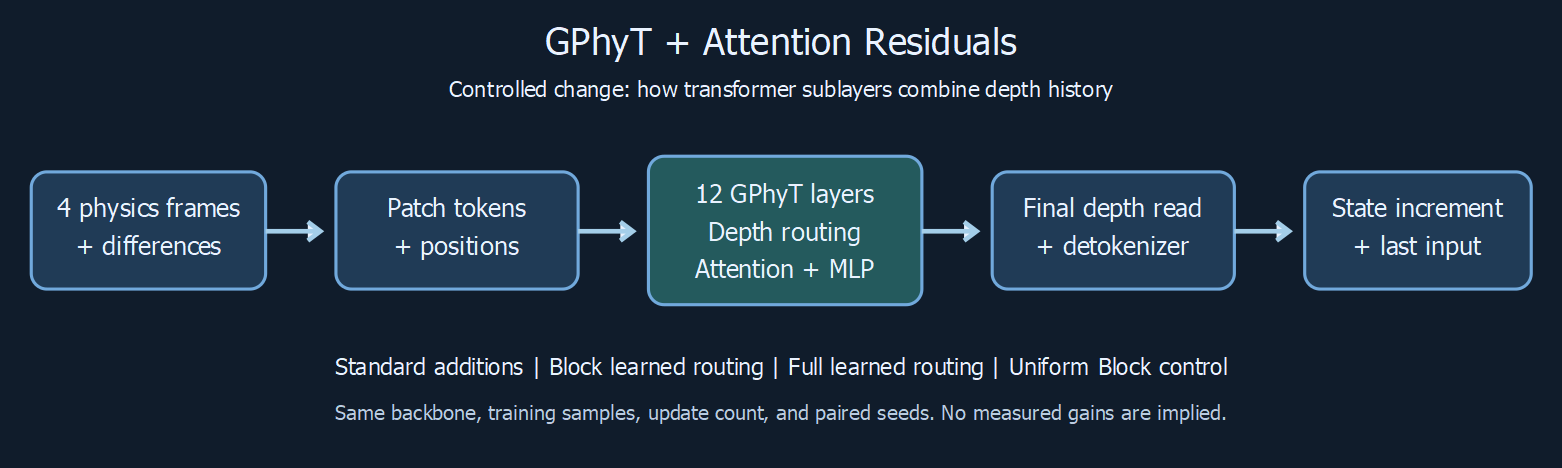
\includegraphics[width=\linewidth]{../reports/figures/architecture.png}
\caption{Controlled architectural change. All variants reuse the same upstream transformations and outer next-state update; only depth composition changes.}
\end{figure}
\subsection{Controlled architecture change}
The backbone has twelve transformer layers, hidden width 192, MLP width 768, three attention heads, absolute positional embeddings, and $1\times16\times16$ spatiotemporal patches. Four context frames at $128\times64$ give 128 tokens. We preserve the upstream tokenizer, positional embeddings, attention, MLPs, finite-difference features, and detokenizer. The upstream forward computes an increment for each context position, adds the original input, and returns the final position. Although the upstream class stores an integrator, this forward does not execute Runge--Kutta integration or use the \texttt{step\_size} argument\cite{gphytcode}.

Write the tokenizer-plus-position output as $e$, and raw attention or MLP output at sublayer $\ell$ as $v_\ell=F_\ell(h_\ell)$. Each $F_\ell$ retains its original normalization. Given the causally available source bank $S_\ell$, our depth read is
\begin{align}
 k_{\ell i} &= \gamma_\ell\odot s_i\left(d^{-1}\sum_{j=1}^{d}s_{ij}^2+10^{-6}\right)^{-1/2},\\
 a_{\ell i} &= \frac{\exp(q_\ell^\top k_{\ell i})}{\sum_{s_r\in S_\ell}\exp(q_\ell^\top k_{\ell r})},
 &h_\ell &=\sum_{s_i\in S_\ell}a_{\ell i}s_i .
\end{align}
These operations apply independently at each token. The query $q_\ell$ starts at zero and the key scale $\gamma_\ell$ at one\cite{attnres,fla}. Mathematically, the initial read is an arithmetic mean, not a sum. Values are the unnormalized sources; only keys are RMS-normalized. There is no additional inverse-square-root attention scale in this operator.

Full routing stores $S_\ell=\{e,v_1,\ldots,v_{\ell-1}\}$. Block routing stores the embedding, completed sums of four consecutive sublayer outputs, and a nonempty partial sum for the current block. A completed sum appears exactly once: its partial slot is cleared at the boundary. Thus the 24 writers form six blocks. A separate final depth read includes all completed outputs before detokenization. The source bank resets for every forward call. Uniform Block uses exactly these sources with fixed equal weights and no learned routing parameters. Standard residuals call the unchanged upstream block forward. With five canonical channels, execution checks count 7,919,045 backbone parameters; learned routing adds $25\times2\times192=9,600$ parameters. This count is specific to our input/output configuration, rather than the parameter count of a differently configured published model.

\subsection{Data and normalization}
The selected datasets originate from Dedalus convection simulations and Athena++ radiative mixing-layer simulations, respectively; we credit their original numerical and physical work\cite{dedalus,fielding} in addition to The Well distribution\cite{well}.
The convection selection fixes Prandtl number 1 and Rayleigh numbers $10^6$, $10^8$, and $10^{10}$. The radiative selection includes all nine cooling settings. Official train, validation, and test trajectory membership is preserved. Source files, coordinates, parameter identities, SHA-256 hashes, and trajectory hashes are recorded before training. Exact full-trajectory duplication across splits causes preparation to fail. Shared initial-state hashes are disclosed separately because identical starting fields need not imply identical trajectories.

Each field is area-downsampled on CPU to $128\times64$ without transposing or reversing stored spatial axes. The canonical channel vector is pressure, density, buoyancy, velocity $x$, and velocity $y$. Buoyancy is not relabeled as temperature. Absent fields are zero, are masked out of optimization and error metrics, and remain zero in autoregressive feedback. Per-dataset, per-active-field means and standard deviations use all selected training trajectories only. Validation/test targets do not enter normalization.

The convection split contains 120 training, 15 validation, and 15 test trajectories; the corresponding radiative counts are 72, nine, and nine. Original grids are $512\times128$ and $128\times384$, with 200 and 101 frames per trajectory. No exact full-trajectory hash crosses splits. There are 33 distinct cross-split first-frame hash groups (25 convection, eight radiative), all spanning different parameter settings; every held-out trajectory shares an initial state with training under another setting. No first-four-frame prepared context is exactly duplicated across splits. This context check is not an exhaustive search over all possible windows. The public manifest and separate audit record all member identities\cite{studycode}.

Training samples are drawn uniformly by dataset, then parameter setting, trajectory, stride in $\{1,\ldots,8\}$, and a valid start index. Four strided context frames predict the fifth. The model receives no explicit parameter label or stride value. Validation monitoring uses a separate fixed sampling generator and cannot advance the training sequence. Evaluation uses stride one and three prespecified start fractions, $0$, $1/2$, and $1$, of the valid origin range for four context plus 24 forecast frames.

\subsection{Optimization and compute allocation}
Under BF16 autocast, the upstream learned FP32 positional embedding promotes the residual stream to FP32. We promote raw sublayer outputs to that same stream dtype before depth-block summation, preserving the standard path's accumulation precision. The attention and MLP matrix operations retain BF16 autocast; this is mixed precision rather than a fully BF16 residual accumulator. Routing also executes inside autocast: FLA's explicit FP32 casts do not prevent its eligible contractions from being autocast\cite{pytorchamp}. The original protocol incorrectly described routing as entirely FP32. This discrepancy was disclosed during training; the frozen training computation was not changed. CPU BF16 regression checks reproduce the distinction; they are not measurements of CUDA rounding error.
Standard and Block variants share seeds 0--5; Full and Uniform Block use seeds 0--2. Backbone initialization is identical within each seed across variants. Data RNGs are independent of model construction and timing, producing paired examples. Standard/Block execution order is randomized within each seed using a fixed scheduling RNG; all primary pairs precede exploratory controls.

Real-data profiling selected microbatch four and froze 3,175 optimizer updates per run, with effective batch sixteen (50,800 sampled examples per run). The fixed cost rule projects 14.400 training hours across all eighteen runs. On the RTX 5070 Laptop GPU with PyTorch 2.14.1+cu130, median update times were 0.7760/0.7913/0.8914/0.8471 seconds for Standard/Block/Full/Uniform, respectively. Each median uses sixteen updates after two warm-ups; these short measurements set the horizon rather than establish a throughput ranking. The profile consumed 71.144 seconds; the previous execution checks consumed 2.920 seconds. The source-linked frozen artifact retains all timings, overhead measurements, hardware identity, sample order, and the portable data fingerprint\cite{studycode}.

All variants use AdamW with learning rate $10^{-4}$, weight decay $10^{-4}$, $(\beta_1,\beta_2)=(0.9,0.999)$, and $\epsilon=10^{-8}$. We clip the accumulated gradient norm to 1, use effective batch size 16, BF16 autocast with FP32 loss reduction, 5\% linear warmup, and cosine decay to $10^{-6}$. A common microbatch is selected from 4, 2, and 1 by memory feasibility. Dropout and stochastic depth remain zero.

The 24 GPU-hour cap allocates 2 hours to profiling/validation, 18 to training, 2 to evaluation, and 2 to contingencies. An exclusive persistent ledger includes failed GPU attempts and wall time spent on IO inside GPU phases. CPU data preparation is outside the GPU allocation. Profiling measures actual optimizer updates for all variants, validation, and checkpoint serialization. A single update count is chosen using measured 90th-percentile update costs, amortized overhead, run multiplicities, and a prespecified 20\% safety margin. This count is published before confirmatory training. The final fixed-update checkpoint defines the endpoint; validation scores never select a better checkpoint.

\subsection{Metrics and statistical analysis}
For standardized target $y$ and prediction $\hat y$, field $c$, and forecast step $t$,
\begin{equation}
 m_{tc}=\frac{\langle(\hat y_{tc}-y_{tc})^2\rangle_{x,y}}{\langle y_{tc}^2\rangle_{x,y}+10^{-6}}.
\end{equation}
For horizon $H$, errors average equally over active fields and steps $1,\ldots,H$, then predetermined windows within a trajectory, then trajectories within each dataset. The target second moment is computed in training-standardized coordinates; this definition is not a claim to reproduce every normalization convention used in The Well benchmarks.

Let $E_{s,d}^{B}$ and $E_{s,d}^{S}$ denote Block and Standard 12-step dataset errors for seed $s$. The independent paired effect is
\begin{equation}
D_s=\tfrac12\sum_{d=1}^{2}\log(E_{s,d}^{B}/E_{s,d}^{S}),\qquad I=1-\exp(\overline D).
\end{equation}
We report all six paired effects, a Student-$t$ interval for $\overline D$ transformed to $I$, and an exact two-sided test enumerating all $2^6$ sign flips. The interval assumes approximately normal independent seed effects; the randomization test requires within-pair exchangeability under its null. Frames and windows are correlated observations, not independent replicates. Inference is conditional on the fixed test trajectories. With six pairs, the minimum two-sided exact p-value is $2/64=0.03125$. Undefined/divergent trajectory errors propagate to dataset estimates; incomplete primary pairs produce an undefined primary analysis rather than a reduced successful-only sample.

Prospective power sensitivity uses assumed Gaussian paired log ratios with standard deviations $0.02$, $0.05$, $0.10$, and $0.20$, and improvements of 5\%, 10\%, and 20\%. It includes noncentral-$t$ power and 100,000 independent simulated exact tests per condition, with simulation RNG seed 20261025. These are assumptions, not estimated post-hoc power.

\subsection{Secondary outcomes and interventions}
Secondary outcomes include one-step and 24-step NMSE, persistence, per-dataset errors, throughput, peak memory, gradient norms, and depth-routing weights. Physical diagnostics include radiative negative-pressure/density fractions and convection velocity-divergence residuals compared with coarsened ground truth using stored physical grid spacing. They do not assert exact conservation or solver equivalence.

On the first four test trajectories per dataset in manifest order, trained Block models are re-evaluated with uniform routing weights and with a fixed-RNG depth permutation of learned weights. These are within-model interventions, not separately retrained models or proof that a mechanism mediates all architecture differences. Their sources and parameters are unchanged; only routing weights are intervened upon. Before test evaluation, an implementation audit replaced the intervention's pointwise FP32 reduction with the same flattened contraction used by ordinary FLA routing. This prevents an additional arithmetic change when weights are held fixed. Exploratory comparisons are reported descriptively without converting secondary tests into a replacement primary endpoint.
